\documentclass{article}
\usepackage{graphicx}
\usepackage[utf8]{inputenc}
\usepackage{fullpage}
\usepackage{listings}
\usepackage{xcolor}
\usepackage{url}
\usepackage[linesnumbered,ruled,vlined]{algorithm2e}
\usepackage{enumitem}


\definecolor{mygreen}{rgb}{0,0.6,0}

% set the default code style
\lstset{
    language=C++,
    frame=tb, % draw a frame at the top and bottom of the code block
    tabsize=4, % tab space width
    showstringspaces=false, % don't mark spaces in strings
    numbers=left, % display line numbers on the left
    commentstyle=\color{mygreen}, % comment color
    keywordstyle=\color{blue}, % keyword color
    stringstyle=\color{red}, % string color
    backgroundcolor=\color{black!5}, % set backgroundcolor
    basicstyle=\footnotesize,% basic font setting
}

\parindent0in
\pagestyle{plain}
\thispagestyle{plain}

\newcommand{\assignment}{Homework 2}
\newcommand{\duedate}{August 5, 2022}


% \renewcommand\thesubsection{\arabic{subsection}}

\title{Homework 2}
\date{}

\begin{document}

Fundação Getulio Vargas\hfill\\
Estruturas de Dados e Algoritmos\hfill\textbf{\assignment}\\
Prof.\ Jorge Poco\hfill\textbf{Due:}: \duedate\\
\smallskip\hrule\bigskip

{\let\newpage\relax\maketitle}
\maketitle


\section{Red-Black Trees}

\textbf{(6pts)} Your job will be to implement a Red-Black Tree in Python. We are providing the file \texttt{red\_black\_tree.py} that you should use as a template for these functions. The functions you will have to implement are: search, insert, remove and print. The last function should print the tree in preorder, indicating if it is a red or black node. For example, for the tree below, the print should show: \texttt{|B-10|B-7|R-16|B-15|B-18|R-30|}

\begin{figure}[h]
  \centering
    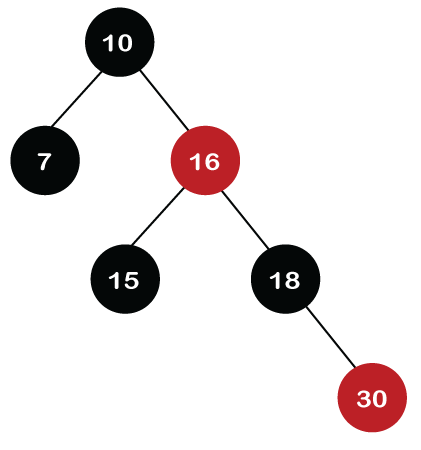
\includegraphics[width=.25\textwidth]{rbt.png}
  % \caption{caption}
  \label{fig:rbt}
\end{figure}


You can find the code on various internet sites, and you are allowed to read and study those resources, but you must write your own code. Also, in the header of the code, you should indicate the websites on which you will rely for the implementation.




To test your code you can follow the examples described in the document \texttt{anexo1.pdf}. In addition, you might be interested in the document \texttt{anexo2.pdf} for a more detailed description of this tree, there is also some Java code that might be useful. 



\section{Sorting in Place in Linear Time}
\textbf{(2pts)} Suppose that we have an array of $n$ data records to sort and that the key of each record has the value 0 or 1. An algorithm for sorting such a set of records might possess some subset of the following three desirable characteristics:

\begin{enumerate}
  \item The algorithm runs in $O(n)$ time.
  \item The algorithm is stable.
  \item The algorithm sorts in place, using no more than a constant amount of storage space in addition to the original array.
\end{enumerate}

\begin{enumerate}[label=(\alph*)]
  \item Give an algorithm that satisfies criteria 1 and 2 above.
  \item Give an algorithm that satisfies criteria 1 and 3 above.
  \item Give an algorithm that satisfies criteria 2 and 3 above.
  \item Can any of your sorting algorithms from parts(a)–(c) be used to sort $n$ records with $b$-bit keys using radix sort in $O(bn)$ time? Explain how or why not.
  \item Suppose that the $n$ records have keys in the range from 1 to $k$. Show how to modify counting sort so that the records can be sorted in place in $O(n + k)$ time. You may use $O(k)$ storage outside the input array. Is your algorithm stable? (Hint: How would you do it for $k = 3$?)

\end{enumerate}

\section{Alternative Quicksort Analysis} 
\textbf{(2pts)} An alternative analysis of the running time of randomized quicksort focuses on the expected running time of each individual recursive call to QUICKSORT, rather than on the number of comparisons performed.

\begin{enumerate}[label=(\alph*)]
  \item Argue that, given an array of size $n$, the probability that any particular element is chosen as the pivot is $1/n$. Use this to define indicator random variables $X_i = I \{i\mbox{th smallest element is chosen as the pivot}\}$. What is $E[X_i]$?
  \item Let $T(n)$ be a random variable denoting the running time of quicksort on an array of size $n$. Argue that
  \begin{equation}
    E[T(n)]=E\left[\sum_{q=1}^{n}X_q(T(q-1)+T(n-q)+\Theta(n))\right]  
    \label{eq:1}
  \end{equation}
  
  \item Show that equation~\ref{eq:1} simplifies to
  \begin{equation}
    E[T(n)] = \frac{2}{n}\sum_{q=0}^{n-1}E[T(q)] + \Theta(n)
    \label{eq:2}
  \end{equation}

  \item Show that
  \begin{equation}
    \sum_{k=1}^{n-1} k \lg k \leq \frac{1}{2}n^2\lg n - \frac{1}{8}n^2
    \label{eq:3}
  \end{equation}
  (Hint: Split the summation into two parts, one for $k=1,2, \ldots, \lceil n/2 \rceil - 1$ and \\ one for $k=\lceil n/2 \rceil~,\ldots,~n-1.)$

  \item Using the bound from equation~\ref{eq:3}, show that the recurrence in equation~\ref{eq:2} has the solution $E[T(n)]=\Theta(n\lg n)$. (Hint: Show, by substitution, that $E[T(n)] \leq an \log n - bn$ for some positive constants $a$ and $b$.)
\end{enumerate}



\end{document}